\documentclass[table]{beamer}
\usepackage[utf8]{inputenc}
\usepackage[brazilian]{babel}
\usepackage{amsmath}
\usepackage{graphicx}
\usepackage{hyperref}
\usepackage{ragged2e}   
\usepackage{epstopdf}
\usepackage{multirow}
\usepackage{minted}
\usepackage{booktabs}

\setbeamertemplate{sidebar right}{}
\setbeamertemplate{footline}{%
\hfill\usebeamertemplate***{navigation symbols}
\hspace{1cm}\insertframenumber{}/\inserttotalframenumber}

\addtobeamertemplate{block begin}{}{\justifying}  %new code

\setbeamertemplate{footline}
{
  \leavevmode%
  \hbox{%
  \begin{beamercolorbox}[wd=.333333\paperwidth,ht=2.25ex,dp=1ex,center]{author in head/foot}%
    \usebeamerfont{author in head/foot}\insertsection
  \end{beamercolorbox}%
  \begin{beamercolorbox}[wd=.333333\paperwidth,ht=2.25ex,dp=1ex,center]{title in head/foot}%
    \usebeamerfont{title in head/foot}\insertsubsection
  \end{beamercolorbox}%
  \begin{beamercolorbox}[wd=.333333\paperwidth,ht=2.25ex,dp=1ex,right]{date in head/foot}%
    \usebeamerfont{date in head/foot}\insertshortdate{}\hspace*{2em}
    \insertframenumber{} / \inserttotalframenumber\hspace*{2ex} 
  \end{beamercolorbox}}%
  \vskip0pt%
}

\begin{document}

\begin{frame}
   \frametitle{Compiladores}
   \large
   \begin{center}
   Análise Sintática Ascendente
   \end{center}
   \scriptsize
   \begin{center}
      João Marcelo Uchôa de Alencar \\
      joao.marcelo@ufc.br \\
      UFC-Quixadá
   \end{center}
\end{frame}

\begin{frame}
   \frametitle{Introdução}
   \begin{itemize}
      \item \textbf{Análise Sintática LR(1)}: entrada processada da esquerda para a direita, mas a derivação produzida é uma derivação à direita, analisando um símbolo da entrada;
      \item \textbf{Análise Sintática LR(0)}: não analisa o símbolo na entrada, apenas quando ele já aparece na pilha;
      \item \textbf{Análise Sintática SLR(1)}: versão melhorada da LR(0), com verificação da entrada;
      \item \textbf{Análise Sintática LALR(1)}: mais poderoso que a SLR(1).
   \end{itemize}
   \begin{center}
   Ordem de complexidade e poder de expressão: \\
   $LR(0) < SLR(1) < LALR(1) < LR(1)$
   \end{center}
   \textbf{Recursão à esquerda} não é um problema para a análise ascendente. Por que?
\end{frame}

\begin{frame}
   \tableofcontents
\end{frame}

\section{Visão Geral}
\begin{frame}[fragile]
   \frametitle{Visão Geral}
   A \textbf{pilha} conterá tanto marcas como não terminais, e também informações adicionais de estados.
   \begin{minted}{text}
$      ...        CadeiaEntrada $
       ...             ...      $
       ...             ...      $
$ SímboloInicial                $ aceita    
   \end{minted}
   Duas operações possíveis:
   \begin{enumerate}
      \item \textbf{Carrega} (\textit{shift}) um terminal do topo da entrada para o topo da pilha;
      \item \textbf{Reduz} (\textit{reduce})  uma cadeia $\alpha$ do topo da pilha para um não terminal A, dada a escolha BNF $A\to\alpha$.
   \end{enumerate}
   As gramáticas são aumentadas com um novo \textbf{símbolo inicial}, com uma única produção unitária para o símbolo inicial anterior.
\end{frame}

\begin{frame}
   \frametitle{Visão Geral - Exemplo}
   $S^{'}\to S$ \\
   $S\to(S)S|\varepsilon$ \\
   \\
   Considerando a cadeia $()$ temos:

   \begin{table}
      \begin{tabular}{|c|l|r|l|}
      \hline
      & Pilha de Análise Sintática & Entrada & Ação \\
      \hline 
      1 & \$        & ()\$ & carrega                         \\
      2 & \$(       &  )\$ & reduz $S\to\varepsilon$         \\
      3 & \$(S      &  )\$ & carrega                         \\
      4 & \$(S)     &   \$ & reduz $S\to\varepsilon$         \\
      5 & \$(S)S    &   \$ & reduz $S\to(S)S$                \\
      6 & \$S       &   \$ & reduz $S^{'}\to S$              \\
      7 & \$$S^{'}$ &   \$ & aceita                          \\
      \hline
      \end{tabular}
   \end{table}
\end{frame}

\begin{frame}
   \frametitle{Visão Geral - Exemplo}
   $E^{'}\to E$ \\
   $E\to E+n|n$ \\
   \\
   Considerando a cadeia $n+n$ temos:

   \begin{table}
      \begin{tabular}{|c|l|r|l|}
      \hline
      & Pilha de Análise Sintática & Entrada & Ação \\
      \hline 
      1 & \$        & n+n\$ & carrega                         \\
      2 & \$n       &  +n\$ & reduz $E\to n$         \\
      3 & \$E       &  +n\$ & carrega                         \\
      4 & \$E+      &   n\$ & carrega   \\
      5 & \$E+n     &    \$ & reduz $E\to E + n$                \\
      6 & \$E       &    \$ & reduz $E^{'}\to E$              \\
      7 & \$$E^{'}$ &    \$ & aceita                          \\
      \hline
      \end{tabular}
   \end{table}
\end{frame}

\begin{frame}
   \frametitle{Visão Geral}
   \begin{itemize}
      \item Um analisador ascendente pode carregar os símbolos de entrada para a pilha até determinar que ação deve executar;
      \item ao mesmo tempo, ele pode precisar de outros elementos da pilha, além do topo, para determinar a ação a ser executada;
      \item \textbf{verificações à frente na pilha}: autômato finito determinístico de \textit{itens};
      \item as verificações na pilha não eliminam a necessidade de analisar a entrada;
      \item a forma em que a verificação é feita é o que difencia o poder e a complexidade dos algoritmos ascendentes.
   \end{itemize}
\end{frame}

\begin{frame}
   \frametitle{Visão Geral - Conceitos}
   Um analisador \textit{shift-reduce} acompanha uma derivação à direita da cadeia, mas os passos ocorrem em ordem inversa:
   \begin{itemize}
      \item \textbf{Forma sentencial à direita}: é uma cadeia intermediária e terminais e não terminais na derivação;
      \item \textbf{prefixo viável}: porção da forma sentencial à direita que está na pilha em um dado momento da derivação;
      \item \textbf{gancho}: cadeia de símbolos no topo da pilha que casa com o lado direito de uma produção $+$ posição na forma sentencial à direita onde ocorre $+$ produção para a redução.
   \end{itemize}
   A tarefa principal de um analisador carrega-reduz é determinar o gancho seguinte em uma análise sintática.
\end{frame}

\section{Análise Sintática LR(0)}
\begin{frame}
   \frametitle{Análise Sintática LR(0)}
   \begin{itemize}
      \item Um \textbf{item LR(0)} de uma gramática livre de contexto é uma escolha de produção com uma posição identificada em seu lado direito; 
      \item se $A\to\alpha$ e $\beta\gamma=\alpha$, $A\to\beta.\gamma$ é um item LR(0). 
   \end{itemize}  
   Para os exemplos: \\
   \begin{columns}
   \begin{column}{0.4\textwidth}
   $S^{'}\to.S$  \\ 
   $S^{'}\to S.$ \\
   $S\to.(S)S$   \\
   $S\to(.S)S$   \\
   $S\to(S.)S$   \\
   $S\to(S).S$   \\
   $S\to(S)S.$   \\
   $S\to.$   \\
   \end{column}
   \begin{column}{0.4\textwidth}
   $E^{'}\to.E$   \\
   $E^{'}\to E.$  \\
   $E\to.E + n$   \\
   $E\to E. + n$  \\
   $E\to E +. n$  \\
   $E\to E + n.$  \\
   $E\to .n$      \\
   $E\to n.$      \\
   \end{column}
   \end{columns}
   \vspace{0.3cm}
   Um item registra um passo intermediário no reconhecimento do lado direito de uma escolha.
\end{frame}

\begin{frame}
   \frametitle{Autômatos Finitos para Itens}
   \begin{block}{Controlar as Opções de Redução}
   Os itens LR(0) podem ser utilizados como os estados de um autômato finito que mantém as informações sobre a pilha de análise sintática e o \textbf{progresso} de uma análise \textit{shift-reduce}.
   \end{block}
   Etapas:
   \begin{enumerate}
      \item Construção de um NFA a partir dos itens;
      \item utilizar a construção de subconjuntos para definir um DFA.
   \end{enumerate}
\end{frame}

\begin{frame}
   \frametitle{Construção de um NFA dos Itens}
    Considere $A\to\alpha\gamma$ e $\gamma$ inicia com $X$ (terminal ou não), tal que $A\to\alpha.X\eta$. Então existe a transição para o item $A\to\alpha X.\eta$: 
   \begin{center}
   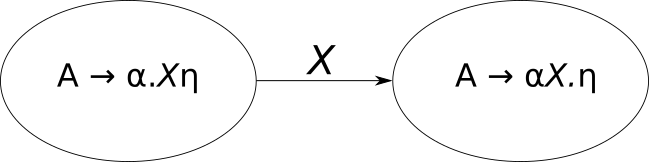
\includegraphics[scale=0.4]{figuras/nfa1.png}
   \end{center}
   Se $X$ for marca, carregar $X$ da entrada para o topo da pilha. Se X for não terminal, ele só pode aparecer por redução. Logo, para $X\to\beta$, $\beta$ deve ser reconhecido \textit{simultaneamente} com a transição acima.
   \begin{center}
   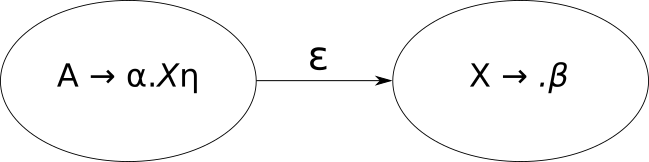
\includegraphics[scale=0.4]{figuras/nfa2.png}
   \end{center}
   Para todas as possibilidades de $\beta$, $X\to\beta$.
\end{frame}

\begin{frame}
   \frametitle{Exemplos}
   Vamos construir os NFAs para os exemplos abaixo. \\
   \begin{columns}
   \begin{column}{0.4\textwidth}
   $S^{'}\to.S$  \\ 
   $S^{'}\to S.$ \\
   $S\to.(S)S$   \\
   $S\to(.S)S$   \\
   $S\to(S.)S$   \\
   $S\to(S).S$   \\
   $S\to(S)S.$   \\
   $S\to.$   \\
   \end{column}
   \begin{column}{0.4\textwidth}
   $E^{'}\to.E$   \\
   $E^{'}\to E.$  \\
   $E\to.E + n$   \\
   $E\to E. + n$  \\
   $E\to E +. n$  \\
   $E\to E + n.$  \\
   $E\to .n$      \\
   $E\to n.$      \\
   \end{column}
   \end{columns}
   \vspace{1.0cm}
   Depois, usar a \textbf{construção de subconjuntos} para transformá-los em DFAs.
\end{frame}

\begin{frame}
   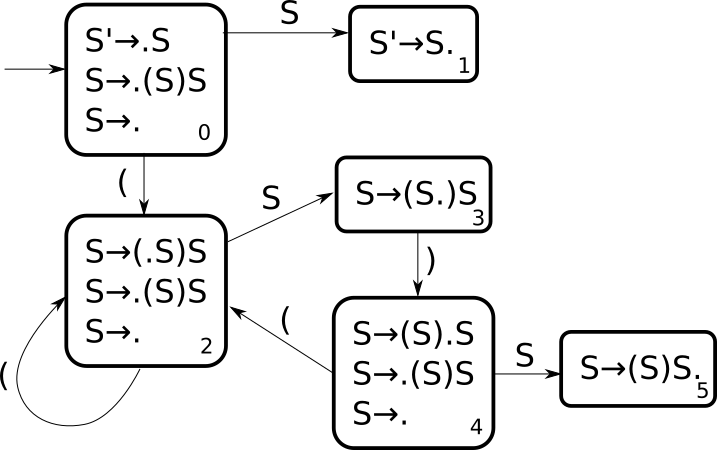
\includegraphics[width=\linewidth,height=\textheight,keepaspectratio]{figuras/ssadfa.png}
\end{frame}

\begin{frame}
   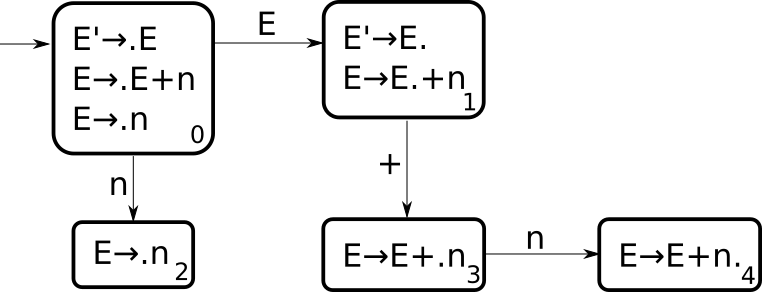
\includegraphics[width=\linewidth,height=\textheight,keepaspectratio]{figuras/endfa.png}
\end{frame}

\begin{frame}
   \frametitle{Definições Adicionais sobre os Autômatos LR(0)}
   \begin{itemize}
      \item \textbf{Itens de fecho}: itens que são adicionados a um estado durante um $\varepsilon$-fecho;
      \item \textbf{itens de núcleo}: itens que geram estados alvos de transições que não são $\varepsilon$-transições.
   \end{itemize}
   Os itens de núcleo determinam de forma única o estado e suas transições.
\end{frame}

\begin{frame}
   \frametitle{O Algoritmo de Análise Sintática LR(0)}
   A pilha passa a conter não apenas símbolos, mas também número de estados. Início:
   \begin{table}
   \begin{tabular}{|l|l|}
   \hline
   Pilha de Análise Sintática & Entrada \\
   \hline 
   \$ 0                       & \textit{CadeiaEntrada} \$ \\
   \hline
   \end{tabular}
   \end{table}
   Carregar a marca $n$ para a pilha e ir para o estado 2:
   \begin{table}
   \begin{tabular}{|l|l|}
   \hline
   Pilha de Análise Sintática & Entrada \\
   \hline 
   \$ 0$n$2                    & \textit{Restante da CadeiaEntrada} \$ \\
   \hline
   \end{tabular}
   \end{table}
   O algoritmo escolhe uma ação com base no estado corrente do DFA, que está no topo da pilha.
\end{frame}

\begin{frame}
   \frametitle{O Algoritmo de Análise Sintática LR(0)}
   Seja $s$ o estado corrente (topo da pilha), ações:
   \begin{enumerate}
      \item Se o estado $s$ contiver um item da forma $A\to\alpha.X\beta$, $X$ terminal, então a \textbf{ação} é carregar a marca da entrada para a pilha. Se a marca for $X$ e $s$ contiver o item $A\to\alpha.X\beta$, então o novo estado a ser empilhado é o que contiver $A\to\alpha X.\beta$. Caso contrário, erro.
      \item Se o estado $s$ contiver um item completo $A\to\gamma.$ então a \textbf{ação} é reduzir por $A\to\gamma$. Uma redução por $S^{'}\to S$ equivale a aceitação, se a entrada estiver vazia. Caso contrário:
      \begin{itemize}
         \item Remover $\gamma$ e os estados correspondentes;
	 \item retorne o DFA para o estado no qual iniciou a construção de $\gamma$;
	 \item o estado atual deve conter item da forma $B\to\alpha.A\beta$;
	 \item coloque $A$ na pilha e atualize o estado para o que contiver $B\to\alpha A.\beta$.
      \end{itemize}
   \end{enumerate}
\end{frame}

\begin{frame}
   \frametitle{Conflitos da Análise Sintática LR(O)}
   Uma gramática é dita LR(0) se as regras anteriores não forem ambíguas. Tipos de conflitoss:
   \begin{itemize}
      \item \textbf{Conflito carrega-reduz}: um estado contém tanto um item $A\to\alpha.$ quanto $A\to\alpha.X\beta$;
      \item \textbf{conflito reduz-reduz}:  um estado contém tanto um item $A\to\alpha.$ quanto $B\to\beta.$;
  \end{itemize}
  Nenhuma das gramáticas apresentadas como exemplo até agora são LR(0). Por quê?
\end{frame}

\begin{frame}
   \frametitle{Exemplo de Gramática LR(0)}
   Para a gramática: \\
   $A\to(A)|a$ \\
   Temos o seguinte autômatos de itens: \\
   \begin{center}
   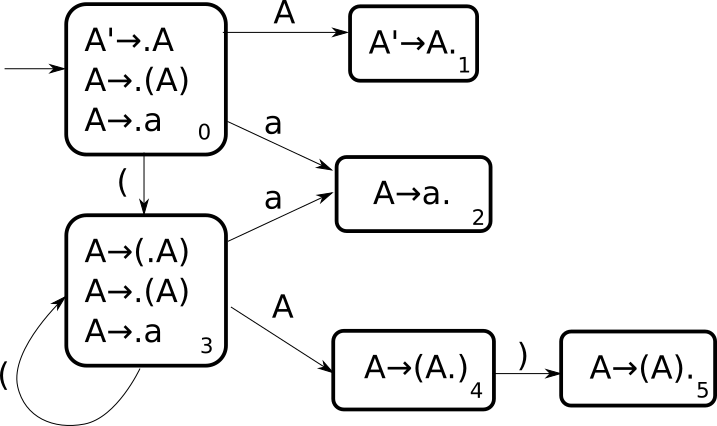
\includegraphics[scale=0.4]{figuras/aadfa.png}
   \end{center}
   Vamos fazer o reconhecimento de ((a))?
\end{frame}

\section{Análise Sintática SLR(1)}
\begin{frame}
   \frametitle{Análise Sintática SLR(1)}
   Vamos aumentar o poder da análise LR(0):
   \begin{enumerate}
      \item Consultar a marca de entrada \textit{antes} de carregar, para garantir que exista uma transição apropriada no DFA;
      \item utilizar o conjunto Sequência de um não-terminal para decidir se uma redução deve ser efetuada.
   \end{enumerate}
\end{frame}

\begin{frame}
   \frametitle{Algoritmo de Análise Sintática SLR(1)}
   Seja $s$ o estado corrente (topo da pilha), ações:
   \begin{enumerate}
      \item Se o estado $s$ contiver um item da forma $A\to\alpha.X\beta$, $X$ terminal, \textbf{e X for a marca seguinte na cadeia de entrada}, então a \textbf{ação} é carregar a marca da entrada para a pilha. O novo estado a ser empilhado é o que contiver $A\to\alpha X.\beta$.
      \item Se o estado $s$ contiver um item completo $A\to\gamma.$, \textbf{e a marca seguinte na cadeia de entrada estiver em Sequência(A)}, então a \textbf{ação} é reduzir por $A\to\gamma$. Uma redução por $S^{'}\to S$ equivale a aceitação, se a entrada for \$. Caso contrário:
      \begin{itemize}
         \item Remover $\gamma$ e os estados correspondentes;
	 \item retorne o DFA para o estado no qual iniciou a construção de $\gamma$;
	 \item o estado atual deve conter item da forma $B\to\alpha.A\beta$;
	 \item coloque $A$ na pilha e atualize o estado para o que contiver $B\to\alpha A.\beta$.
      \end{itemize}
      \item Se a marca de entrada for tal que nenhum caso acima se aplique, erro!
   \end{enumerate}
\end{frame}

\begin{frame}
   \frametitle{Conflitos da Análise Sintática SLR(1)}
   Dizemos que uma gramática é SLR(1) se a aplicação das regras não resultarem em ambiguidade. As duas condições devem ser satisfeitas:
   \begin{enumerate}
      \item Para qualquer item $A\to\alpha.X\beta$ em $s$ em que $X$ for um não terminal, não existe um item completo $B\to\gamma.$ em $s$ com X em Sequência(B);
      \item Para quaisquer dois itens completos $A\to\alpha.$ e $B\to\beta.$ em $s$, Sequência(A) $\cap$ Sequência(B) é vazio.
   \end{enumerate}
   A violação da primeira condição representa um \textbf{conflito carrega-reduz}. A violação da segunda condição representa um \textbf{conflito reduz-reduz}.
\end{frame}

\begin{frame}
   \frametitle{Construção da Tabela SLR(1)}
   Percorrendo o autômato gerado, considerando cada terminal e não-terminal, podemos construir a tabela SLR(1). Dada a gramática \\
   $E^{'}\to E$ \\
   $E\to E+n|n$ \\
   e o autômato gerado para ela e o fato de que Sequência(E)$=\{\$\}$ e Sequência(E')$=\{\$,+\}$, temos a tabela:
   \begin{table}
   \begin{tabular}{|c|c|c|c|c|}
   \hline
   \textbf{Estado} & \multicolumn{3}{c|}{\textbf{Entrada}} & \textbf{Ir-para}\\
   \hline 
   & $n$ & $+$ & \$ & $E$  \\
   \hline
   0 & s2 &               &               & 1 \\
   1 &    & s3            & aceita        & \\
   2 &    & r($E\to n$)   & r($E\to n$)   & \\
   3 & s4 &               &               & \\
   4 &    & r($E\to E+n$) & r($E\to E+n$) & \\
   \hline
   \end{tabular}
   \end{table}
   Vamos fazer a análise da cadeia $n+n+n$.
\end{frame}

\begin{frame}
   \frametitle{Regras para Eliminar Ambiguidades}
   No caso da SLR(1), podemos tomar algumas atitudes para eliminar ambiguidades:
   \begin{itemize}
      \item No caso dos conflitos carrega-reduz, existe uma regra natural, que é sempre preferir carregar em vez de reduzir;
      \item o caso dos conflitos reduz-reduz, não há solução geral, geralmente é indício de erro no projeto.
   \end{itemize}
   A solução de carregar no lugar de reduzir tem algum impacto no problema do \textit{else} aninhado?
\end{frame}

\begin{frame}
   \frametitle{Exemplo de Eliminação de Ambiguidade}
   Considere a gramática: \\
   \\
   $\textit{declaração}\to \textit{if-decl}|\textbf{outra}$ \\
   $\textit{if-decl} \to \textbf{if}(exp) \textit{declaração}$ \\
   $|\textbf{if}(exp)\textit{declaração }\textbf{else }\textit{declaração}$ \\
   $exp\to\textbf{0}|\textbf{1}$ \\
   \\
   É notoriamente ambígua. Vamos simplificá-la para poder criar o autômato: \\
   \\
   $S\to I|\textbf{outra}$ \\
   $\textbf{I}\to\textbf{if }S|\textbf{if }S\textbf{ else }S$ \\
   \\
   Temos a seguinte propriedade: \\
   Sequência($S$) = Sequência($I$) = $\{\$, else\}$
\end{frame}

\begin{frame}
   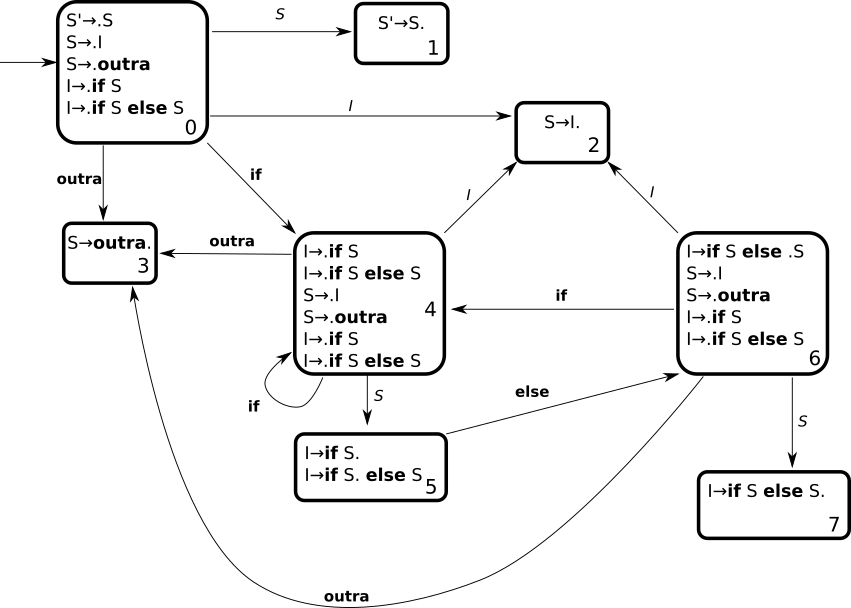
\includegraphics[width=\linewidth,height=\textheight,keepaspectratio]{figuras/ifthenelsedfa.png}
\end{frame}

\begin{frame}
   \frametitle{Exemplo de Eliminação de Ambiguidade}
   O estado 5 tem $\{I\to\textbf{if }S.\text{;}I\to\textbf{if }S.\textbf{ else }S\}$.
   \begin{itemize}
      \item Devemos reduzir nas entradas \textbf{else} e \$ na primeira derivação?
      \item ou devemos  apenas carregar o \textbf{else} na segunda derivação?
   \end{itemize}
   \begin{table}
      \begin{tabular}{|c|c|c|c|c|c|c|}
      \hline
      \textbf{Estado} & \multicolumn{4}{c|}{\textbf{Entrada}} & \multicolumn{2}{c|}{\textbf{Ir-para}} \\
      \hline 
       & if & else & outra & \$ & S & I \\
       \hline
       0 & s4 &    & s3 &        & 1 & 2 \\
       1 &    &    &    & aceita &   &   \\
       2 &    & r1 &    & r1     &   &   \\
       3 &    & r3 &    & r2     &   &   \\
       4 & s4 &    & s3 &        & 5 & 2 \\
       5 &    & \textbf{s6} &    & r3     &   &   \\
       6 & s4 &    & s3 &        & 7 & 2 \\
       7 &    & r4 &    & r4     &   &   \\
      \hline
      \end{tabular}
   \end{table}
\end{frame}

\begin{frame}
   \frametitle{Limitações da Análise SLR(1)}
   \begin{columns}
   \begin{column}{0.5\textwidth}
   \small
   $decl\to \textit{ativação-decl}|\textit{atribuição-decl}$ \\
   $\textit{ativação-decl}\to \textbf{identificador}$ \\
   $\textit{atribuição-decl}\to var:=exp$ \\
   $var \to var[exp] | \textbf{identificador}$ \\
   $exp \to var | \textbf{número}$ \\
   \vspace{1.0cm}
   Tanto as atribuições quanto declarações começam com \textbf{identificador}.
   \end{column}
   \begin{column}{0.5\textwidth}
   \small
   Versão simplificada: \\
   $S \to \textbf{id}|V:=E$ \\
   $V \to \textbf{id}$ \\
   $E \to V|\textbf{n}$ \\
   Considere o estado inicial com os itens: \\
   $S^{'} \to .S$ \\
   $S \to .\textbf{id}$ \\
   $S \to .V := E $ \\
   $V \to .\textbf{id}$ \\
   \vspace{1.0cm}
   Há conflito para os terminais \textbf{id}.
   \end{column}
   \end{columns}
   \begin{block}{Algoritmos SLR(k)}
   Considerar algoritmos SLR(k) aumenta a expressividade para esses casos, mas a \textbf{complexidade} se torna intratável.
   \end{block}
\end{frame}

\section{Análise Sintática Geral LR(1) e LALR(1)}
\begin{frame}
   \frametitle{Análise Sintática Geral LR(1) e LALR(1)}
   \begin{itemize}
      \item Podemos resolver o problema anterior com a análise LR(1) \textbf{canônica};
      \item essa análise torna o processo complexo devido ao tamanho do autômato gerado;
      \item uma modificação, LALR(1), permite condensar alguns estados em um autômato menor;
      \item entretanto, para compreender a LALR(1), precisamos entender a LR(1) antes.
   \end{itemize}
\end{frame}

\begin{frame}
   \frametitle{Autômatos Finitos de Itens LR(1)}
   O poder do método LR(1) geral é ele utilizar um DFA novo com as verificações à frente construídas em sua concepção.
   \begin{itemize}
      \item \textbf{Item LR(1)}: par composto por um item LR(0) e uma marca de \textit{verificação à frente};
      \item $[A\to\alpha.\beta, a]$, onde $A\to\alpha.\beta$ é um item LR(0) e $a$ é uma marca. Não é a marca à frente na entrada, mas sim uma informação sobre o que se espera na entrada após uma redução.
   \end{itemize}
   A maior diferença entre os autômatos LR(0) e LR(1) aparece na definição das $\varepsilon$-transições.
\end{frame}

\begin{frame}
   \frametitle{Transições dos Autômatos LR(1)}
   \begin{block}{Transições Determinísticas}
   Dado um item LR(1) $[A\to\alpha.X\gamma,a]$, onde $X$ é qualquer símbolo (terminal ou não), existe uma transição em X para o item LR(1) $[A\to\alpha X.\gamma, a]$. \textbf{Não há mudança no símbolo de verificação}.
   \end{block}

   \begin{block}{Transições $\varepsilon$}
   Dado um item LR(1) $[A\to\alpha.B\gamma,a]$, onde \textbf{B é um não terminal}, existem $\varepsilon$-transições $[B\to.\beta, b]$ para cada produção $B \to \beta$ e cada \textbf{marca} $b$ pertencente a Primeiro($\gamma$a).
   \begin{itemize}
      \item $[A\to\alpha.B\gamma,a]$ indica que reconhecemos B se após ocorrer uma cadeia \textit{derivável} de $\gamma a$, começando por marcas presentes em Primeiro($\gamma a$);
      \item restringimos as capturas à conjuntos $Primeiro$, não $Sequencia$;
      \item a verificação original $a$ só é propagada se $\gamma \Rightarrow \varepsilon$.
   \end{itemize}
   \end{block}
\end{frame}

\begin{frame}
   \frametitle{Exemplo de Autômato LR(1)}
   Considere a gramática: \\
   $A\to(A)|a$ \\
   Vamos construir o autômato LR(1)?
\end{frame}

\begin{frame}
   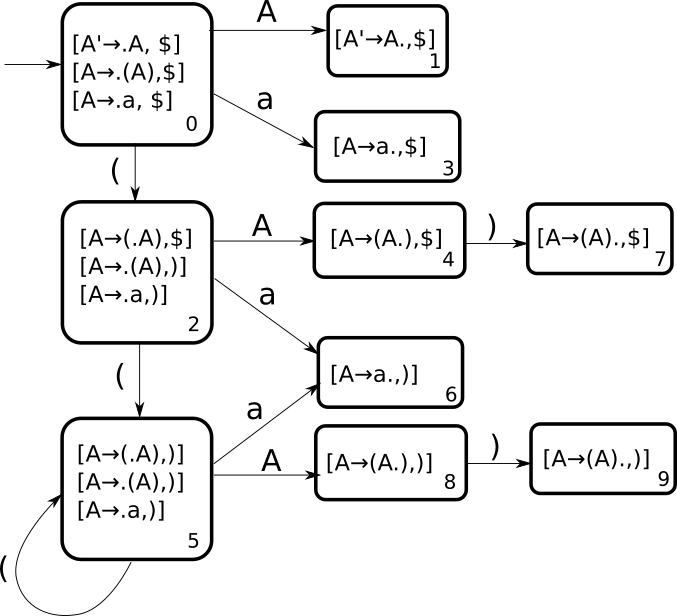
\includegraphics[width=\linewidth,height=\textheight,keepaspectratio]{figuras/aadfalr1.png}
\end{frame}

\begin{frame}
   \frametitle{Tabela LR(1)}
   Enumeramos as produções da gramática:
   \begin{enumerate}
      \item $A\to(A)$
      \item $A\to a$
   \end{enumerate}
   \begin{table}
      \begin{tabular}{|c|c|c|c|c|c|}
      \hline
      \textbf{Estado} & \multicolumn{4}{c|}{\textbf{Entrada}} & \textbf{Ir-para} \\
      \hline 
         & (  & a  & )  & \$     & A  \\
       \hline
       0 & s2 & s3 &    &        & 1  \\
       1 &    &    &    & aceita &    \\
       2 & s5 & s6 &    &        & 4  \\
       3 &    &    &    & r2     &    \\
       4 &    &    & s7 &        &    \\
       5 & s5 & s6 &    &        & 8  \\
       6 &    &    & r2 &        &    \\
       7 &    &    &    & r1     &    \\
       8 &    &    & s9 &        &    \\
       9 &    &    & r1 &        &    \\
      \hline
      \end{tabular}
   \end{table}
\end{frame}

\begin{frame}
   \frametitle{Algoritmo de Análise Sintática LR(1) Geral}
   Seja $s$ o estado corrente (topo da pilha), ações:
   \begin{enumerate}
      \item Se o estado $s$ contiver um item LR(1) da forma $[A\to\alpha.X\beta, a]$, $X$ terminal, \textbf{e X for a marca seguinte na cadeia de entrada}, então a \textbf{ação} é carregar a marca da entrada para a pilha. O novo estado a ser empilhado é o que contiver $[A\to\alpha X.\beta,a]$.
      \item Se o estado $s$ contiver um item completo LR(1) [$A\to\alpha.,a]$, \textbf{e a marca seguinte na entrada for $a$}, então a \textbf{ação} é reduzir por $A\to\alpha$. Uma redução por $S^{'}\to S$ equivale a aceitação, se a entrada for \$. Caso contrário:
      \begin{itemize}
         \item Remover $\alpha$ e os estados correspondentes;
	 \item retorne o DFA para o estado no qual iniciou a construção de $\alpha$;
	 \item o estado atual deve conter item da forma $[B\to\alpha.A\beta, b]$;
	 \item coloque $A$ na pilha e atualize o estado para o que contiver $[B\to\alpha A.\beta, b]$.
      \end{itemize}
      \item Se a marca de entrada for tal que nenhum caso acima se aplique, erro!
   \end{enumerate}
\end{frame}

\begin{frame}
   \frametitle{Requisitos para uma Gramática LR(1)}
   Uma gramática é LR(1) se e somente se, para qualquer estado $s$, as seguintes duas condições forem satisfeitas:
   \begin{enumerate}
      \item Para qualquer item $[A\to\alpha.X\beta, a]$ pertencente a $s$ em que $X$ é um terminal, não existe um item pertencente a $s$ da forma $[B\to\gamma.,X]$ (carrega-reduz);
      \item não há dois itens em $s$ da forma $[A\to\alpha.,a]$ e $[B\to\beta., a]$ (reduz-reduz).
   \end{enumerate}
\end{frame}

\begin{frame}
   \frametitle{Exemplo de Gramática LR(1)}
   Considere o exemplo problemático para SLR(1): \\
   $S \to \textbf{id}|V:=E$ \\
   $V \to \textbf{id}$ \\
   $E \to V|\textbf{n}$ \\
   Vamos construir o autômato LR(1)?
\end{frame}

\begin{frame}
   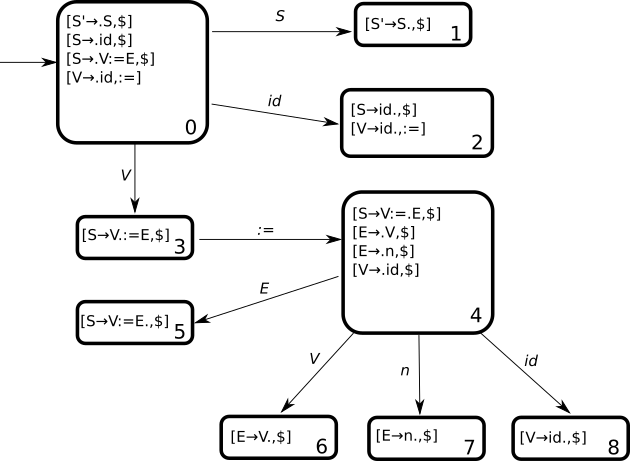
\includegraphics[width=\linewidth,height=\textheight,keepaspectratio]{figuras/iddfalr1.png}
\end{frame}

\begin{frame}
   \frametitle{Análise Sintática LALR(1)}
   \begin{itemize}
      \item O tamanho do DFA LR(1) se deve à existência de estados com o mesmos itens LR(0), mas com símbolos de verificação diferentes;
      \item a análise LALR(1) identifica tais estados e os combina;
      \item agora, o estado LALR(1) não tem um símbolo de verificação, mas sim um conjunto deles;
      \item \textbf{núcleo} de um estado LR(1): conjunto de itens LR(0) composto pelos primeiros componentes de todos os itens LR(1) no estado.
   \end{itemize}
\end{frame}

\begin{frame}
   \frametitle{Princípios da Análise Sintática LALR(1)}
   \begin{block}{Primeiro Princípio da Análise Sintática LALR(1)}
   O núcleo de um estado do DFA de itens LR(1) é um estado DFA de itens LR(0).
   \end{block}
 
   \begin{block}{Segundo Princípio da Análise Sintática LALR(1)}
   Dados dois estados $s_{1}$ e $s_{2}$ do DFA de itens LR(1) com o mesmo núcleo, suponha que exista uma transição em $X$ de $s_{1}$ para um estado $t_{1}$. Portanto, existe também uma transição em X do estado $s_{2}$ para o estado $t_{2}$, e os estados $t_{1}$ e $t_{2}$ têm o mesmo núcleo.
   \end{block}
   \textbf{DFA de itens LALR(1)}: a partir do autômato LR(1), identificar todos os estados com o mesmo núcleo e unir todos os símbolos de verificação correspondentes a um item LR(0) em um conjunto.
\end{frame}

\begin{frame}
   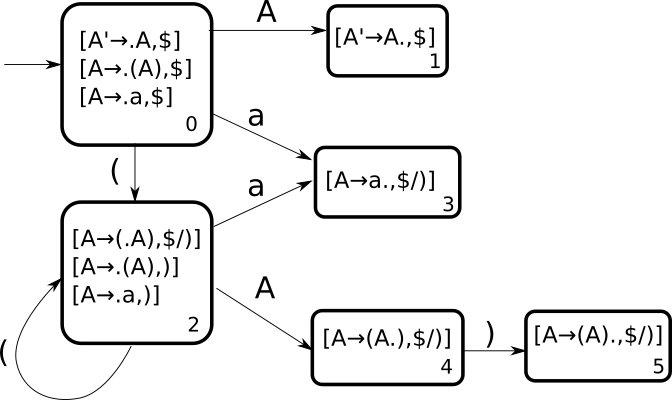
\includegraphics[width=\linewidth,height=\textheight,keepaspectratio]{figuras/aadfalalr1.png}
\end{frame}

\begin{frame}
   \frametitle{Consequências da Análise LALR(1)}
   \begin{itemize}
      \item O algoritmo para análise LALR(1) é o mesmo usado na LR(1);
      \item é possível que a transformação do autômato em LALR(1) cause conflitos inexistentes no autômato LR(1);
      \item na maioria das construções de linguagens de programação, esses conflitos não ocorrem;
      \item a \textbf{propagação de verificações à frente} permite computar o autômato LALR(1) diretamente a partir do autômato LR(0).
   \end{itemize}
\end{frame}

\section{YACC}

\begin{frame}
   \frametitle{YACC - \textit{Yet Another Compiler Compiler}}
   \begin{block}{Gerador de Analisadores Sintáticos}
      Programa que recebe como entrada uma especificação da sintaxe de uma linguagem e produz como saída um procedimento de análise sintática para aquela linguagem. \\ 
   \end{block}
   \begin{itemize}
      \item \textbf{Compilador de compiladores};
      \item algoritmo LALR(1);
      \item Várias versões;
      \item funciona com C/C++.
   \end{itemize}
\end{frame}

\begin{frame}[fragile]
   \frametitle{YACC - \textit{Yet Another Compiler Compiler}}
   \begin{block}{Instalar a versão Ubuntu:}
      \$ sudo apt install bison
   \end{block}
   \begin{block}{Arquivos de especificação \textbf{.y} com a gramática e ações:}
      \begin{minted}{bash}
      {definições}
      %%
      {regras}
      %%
      {rotinas auxiliares}
      \end{minted}
   \end{block}
   São gerados os arquivos \textit{y.tab.c} e \textit{y.tab.h} para arquivo de entrada da gramática.
\end{frame}

   \begin{frame}
   \frametitle{Definições}
   \begin{itemize}
      \item Marcas e tipos de dados necessários para a geração do analisador sintático;
      \item as marcas são constantes inteiras definidas que devem corresponder às marcas geradas pelo analisador léxico;
      \item você pode recortar e colar essas marcas nos dois cabeçalhos, ou incluir o arquivo de cabeçalho gerado pelo \textit{yacc} nos arquivos gerados pelo \textit{lex}.
      \item também nesta seção está o código em C que deve ser inserido diretamente no analisador sintático:
      \begin{itemize}
         \item funções auxiliares;
         \item diretivas \#include.
      \end{itemize}
      \item toda a seção de Definições pode estar vazia se o objetivo for apenas estudar a geração da tabela.
   \end{itemize}
\end{frame}

\begin{frame}
   \frametitle{Regras}
   \begin{itemize}
      \item São as regras da gramática em BNF adaptada;
      \item para cada regra pode existir uma \textbf{ação} associada:
      \begin{itemize}
         \item ações são código em C que é executado toda vez que o analisador LALR(1) realiza uma \textbf{redução} na regra associada;
         \item em teoria esse código pode ser qualquer coisa, inclusive a construção de uma árvore sintática.
      \end{itemize}
      \item como não há o símbolo $\rightarrow$ na maioria dos teclados, usamos : em seu lugar;
      \item a regra gramatical termina sempre com ponto e vírgula. 
   \end{itemize}
\end{frame}

\begin{frame}
   \frametitle{Rotinas Auxiliares}
   \begin{itemize}
      \item Rotinas auxiliares e declarações de funções;
      \item código que o desenvolvedor optou por não incluir em um cabeçalho (no caso, seria incluso na seção de Definições);
      \item pode ser vazia, eliminando a necessidade do segundo símbolo de separação \%\%;
      \item os comentários em estilo C são permitidos aqui, assim como nas Regras e Definições.
   \end{itemize}
\end{frame}

\begin{frame}
   \frametitle{Exemplo Básico - Gramática de Parênteses}
   Considere a gramática mais simples que usamos nos exemplos: \\
   A $\rightarrow$ (A) \\
   A $\rightarrow$ a\\
   Vamos criar um arquivo de entrada para o \textit{yacc} reconhecer cadeias desta gramática: \\
   \begin{itemize}
      \item Só tem três \textit{tokens}: (, a e );
      \item portanto, vamos fazer a análise léxica manualmente.
   \end{itemize}
\end{frame}

\begin{frame}[fragile]
   \frametitle{Arquivo \textit{src/yacc/parenteses/parenteses.y}}
   Seções \textbf{Definições} e \textbf{Regras}:
   \scriptsize
   \begin{minted}{c}
%{
#include <stdio.h>
#include <ctype.h>
int yylex(void);
int yyerror(char *);
%}

%token LPARAM RPARAM LITTLEA

%%

A : LPARAM A RPARAM { printf("Fazendo redução por A -> (A).\n"); }
   | LITTLEA        { printf("Fazendo redução por A -> a.\n"); }
   ;

%%
   \end{minted}
\end{frame}

\begin{frame}[fragile]
   \frametitle{Arquivo \textit{src/yacc/parenteses/parenteses.y}}
   Seção \textbf{Rotinas Auxiliares}:
   \scriptsize
   \begin{minted}{c}
int main(int argc, char *argv[]) {
   return yyparse();
}

int yylex(void) {
   int c;

   while ((c = getchar()) == ' ');

   if (c == '(' ) return LPARAM;
   else if (c == ')') return RPARAM;
   else if (c == 'a') return LITTLEA;
   else if (c == '\n') return 0; 
   return c; 
}

int yyerror(char *s) {
   fprintf(stderr, "%s\n", s);
   return 0;
}
   \end{minted}
\end{frame}

\begin{frame}[fragile]
   \frametitle{Geração da Tabela e Compilação do Analisador}
   \begin{minted}{bash}
      $ yacc parenteses.y
      $ gcc yy.tab.c -o parenteses
      $ ./parenteses
      ((a))
      Fazendo redução por A -> a.
      Fazendo redução por A -> (A).
      Fazendo redução por A -> (A).
   \end{minted}
   Criamos os \textit{tokens} LPARAM, RPARAM e LITTLEA. Mas para símbolos de um único caracteres, podemos inseri-los entre aspas:
   \begin{minted}{c}
   A : '(' A ')'
     | 'a'
     ;
   \end{minted}
   Para cenários mais complexos (identificadores, números, etc), precisamos criar os \textit{tokens}.
\end{frame}

\begin{frame}
   \frametitle{Opções \textit{yacc}}
   Se quisermos que as funções geradas pelo \textit{yacc} e outras definições (como as marcas para o \textit{lex}) estejam disponíveis em um cabeçalho:
   \begin{itemize}
      \item \$ yacc -d parenteses.y
      \item arquivo \textit{y.tab.h} é criado.
   \end{itemize}
   É possível gerar uma descrição textual do autômato LALR(1):
   \begin{itemize}
      \item \$ yacc -v parenteses.y
      \item o arquivo \textit{y.output} é criado;
      \item os estados contém apenas os itens de \textbf{núcleo}.
      \item as transições indicam as ações do analisador e o contéudo da tabela IR-PARA.
   \end{itemize}
   Compare o conteúdo do arquivo com Figura 5.9 do livro. 
   
\end{frame}

\begin{frame}
   \frametitle{Gramática de Expressões Ariméticas para o YACC}
   Vamos estudar um exemplo um pouco mais robusto: \\
   $exp\to\textit{exp soma termo}|termo$ \\
   $soma\to+|-$ \\
   $termo\to\textit{termo mult fator}|fator$ \\
   $mult\to *$ \\
   $fator\to(exp)|\textbf{número}$\\
   Esta gramática foi usada como exemplo em vários capítulos. 
\end{frame}

\begin{frame}[fragile]
   \frametitle{Definições - arquivo \textit{src/yacc/aritmetica/aritmetica.y}}
   \begin{minted}{c}
%{
#include <stdio.h>
#include <ctype.h>

int yylex(void);
int yyerror(char *);
%}

%token NUMBER
  \end{minted}
\end{frame}

\begin{frame}[fragile]
   \frametitle{Regras - arquivo \textit{src/yacc/aritmetica/aritmetica.y}}
   \begin{minted}{perl}
%%
command : exp { printf("%d\n", $1); }
        ; /* permite imprimir o resultado */

exp : exp '+' term { $$ = $1 + $3; }
    | exp '-' term { $$ = $1 + $3; }
    | term { $$ = $1; }
    ;
 
term : term '*' factor { $$ = $1 * $3; }
     | factor { $$ = $1 ;} 
     ;

factor : NUMBER { $$ = $1; }
       | '('exp')' { $$ = $2; }
       ;

   \end{minted}
\end{frame}

\begin{frame}[fragile]
   \frametitle{Rotinas Auxiliares - \textit{src/yacc/aritmetica/aritmetica.y}}
   \scriptsize
   \begin{minted}{c}
%%

int main() {
   return yyparse();
}

int yylex(void) {
   int c;
   while ((c=getchar()) == ' '); /* elimina espaços em branco */
   if (isdigit(c)) {
      ungetc(c,stdin);
      scanf("%d", &yylval);
      return(NUMBER);
   }
   if (c == '\n') return 0; /* interrompe a análise sintática */
   return c;
}

/* imprimir a mensagem erro */
int yyerror(char *s) {
   fprintf(stderr, "%s\n", s);
   return 0;
}
   \end{minted}

\end{frame}

\begin{frame}
   \frametitle{Gramática de Expressões Ariméticas para o YACC}
   \begin{itemize}
      \item O único \textit{token} (NUMBER) é apresentado nas definições;
      \item os outros terminais são inclusos diretamente na gramática, entre aspas simples (os operadores);
      \item temos um novo símbolo inicial, \textsf{command}, para deixar a definição do autômato LALR(1) mais organizada;
      \item as ações fazem uso de \textbf{pseudovariáveis}:
      \begin{itemize}
         \item quando ocorre uma redução por uma regra, o \textit{yacc} atribui um \textbf{valor} a cada não-terminal da regra;
         \item por padrão, esse \textbf{valor} é inteiro, mas pode ser qualquer tipo em C/C++, inclusive ponteiros, estruturas, etc;
         \item o \textit{yacc} mantém uma \textbf{pilha de valores}, em paralelo com a pilha de análise sintática.
      \end{itemize}
   \end{itemize}
\end{frame}

\begin{frame}[fragile]
   \frametitle{Pseudovariáveis}
   Considere a regra e ação associada:
   \begin{minted}{perl}
   exp : exp '+' termo {$$ = $1 + $3;}
   \end{minted}
   \begin{itemize}
      \item O símbolo \$ indica um valor da pilha de valores;
      \item o símbolo \$\$ representa o símbolo à esquerda na regra gramatical;
      \item As variáveis \$1, \$2, \$3 indicam os valores dos símbolos na primeira, segunda e terceira posição, do lado direito;
      \item no caso, não existe valor para o segundo símbolo, '+, uma marca terminal;
   \end{itemize}
   Neste exemplo, estamos afirmando que o valor da expressão que estará pilha após a redução é igual a soma do valor da expressão do lado direito e termo.
\end{frame}


\begin{frame}[fragile]
   \frametitle{Pseudovariáveis}
   Considere a regra e ação associada:
   \begin{minted}{perl}
   factor : NUMBER {$$ = $1;}
   \end{minted}
   \begin{itemize}
      \item Neste caso, NUMBER é um terminal, com valor (\$1);
      \item o analisador léxico deve retornar o valor de NUMBER preenchendo a variável \textit{yylval} quando a marca é reconhecida;
      \item a \textit{yylval} deve ser ma variável global compartilhada entre o análisado léxico e o sintático.
   \end{itemize}
   Você pode considerar que \textit{yylval} seria o lexema ou um outro atributo da marca.
\end{frame}

\begin{frame}
   \frametitle{Rotinas Auxiliares}
   \begin{itemize}
      \item A função \textit{main} ativa \textit{yyparse()}, que retorna 0 em sucesso da análise sintática, 1 caso contrário;
      \item implicitamente, \textit{yyparse()} invoca uma função \textit{yylex()} que pode ter sido criada pelo \textit{lex};
      \item no exemplo, \textit{yylex()} foi feita manualmente, vale observar como \textit{yylval} é preenchida;
      \item temos também a função \textit{yyerror()}, apenas imprimindo uma mensagem de erro.
   \end{itemize}
\end{frame}

\begin{frame} [fragile]
   \frametitle{Gerando o Autômato LALR(1) para Expressões Aritméticas}
   Arquivo simplicado, sem as ações e rotinas auxiliares:
   \scriptsize
   \begin{minted}{perl}
      %token NUMBER
      %% 
      command : exp
               ; 
      exp : exp '+' term 
               | exp '-' term 
               | term 
               ;
      term : term '*' factor 
               | factor 
               ;      
      factor : NUMBER 
               | '('exp')' 
               ;  
   \end{minted}
   \normalsize
   \$ yacc -v aritmetica\_simplicada.y \\
   Teremos o arquivo \textit{y.output} com o autômato LALR(1). Sem as ações e rotinas, fica mais fácil visualizar as transições dos estados.
\end{frame}

\begin{frame}[fragile]
   \frametitle{Depurando a Execução do Analisador Sintático}
   Adicionar:
   \begin{minted}{perl}
   #define YYDEBUG 1
   \end{minted}
   na seção de Definições, e:
   \begin{minted}{perl}
   extern int yydebug;
   yydebug = 1;
   \end{minted}
   no começo da função \textit{main}. Agora basta gerar o executável novamente, informando entrada. 
\end{frame}

\begin{frame}
   \frametitle{Conflitos e Eliminação de Ambiguidade}
   \begin{itemize}
      \item O \textit{yacc} tem regras internas para eliminar ambiguidade;
      \item o arquivo \textit{y.output} permite verificar se essas regras surtiram efeito;
      \item conflitos \textbf{carrega-reduz} são resolvidos para opção carregar;
      \item conflitos \textbf{reduz-reduz} tem a ambiguidade eliminada pela precedência da redução da regra que aparece primeiro no arquivo de especificação.
   \end{itemize}
   Considere a gramática visivelmente ambígua: \\
   A $\rightarrow$ A $|$ B \\
   A $\rightarrow$ a \\
   B $\rightarrow$ a \\
   Gere o arquivo \textit{y.output} dela.
\end{frame}

\begin{frame}[fragile]
   \frametitle{Precedência de Operadores e Associatividade}
   \scriptsize
   \begin{minted}{bash}
   %{
   #include <stdio.h>
   #include <ctype.h>
   %}

   %token NUMBER
   
   %left '+' '-'
   %left '*'

   %%
   command : exp { printf("%d\n", $1); }
           ;
   exp     : NUMBER { $$ = $1 ;}
           | exp '+' exp { $$ = $1 + $3 ;}
           | exp '-' exp { $$ = $1 - $3 ;}           
           | exp '*' exp { $$ = $1 * $3 ;}           
           | '(' exp ')' { $$ = $2;}
           ;
   %%
   /* Mesmas funções auxiliares do outro exemplo. */
   \end{minted}
\end{frame}

\begin{frame}[fragile]
   \frametitle{Precedência de Operadores e Associatividade}
   As linhas abaixo:
   \begin{minted}{bash}
   %left '+' '-'
   %left '*'
   \end{minted}
   Indicam que os operadores + e - têm a mesma precedência e são associativos à esquerda. O operador * é associativo à esquerda e tem precedência maior que os outros. Os operadores \%right e \%nonassoc também estão disponíveis.
\end{frame}

\begin{frame}[fragile]
   \frametitle{Tipos de Valores Arbitrários}
   \begin{itemize}
      \item No exemplo da gramática de expressões aritmeticas, as pseudovariáveis tem valor inteiro (o padrão);
      \item mas se quisessemos calcular operações de ponto flutuante?
      \item ou melhor, se quisessemos construir a árvore sintática durante a derivação?
      \item podemos redefinir o tipo das pseudovariáveis usando o símbolo YYSTYPE:
   \end{itemize}
   \begin{minted}{perl}
      #define YYSTYPE double
   \end{minted}
\end{frame}

\begin{frame}[fragile]
   \frametitle{Tipos de Valores Arbitrários}
   Considere a gramática: \\
   exp $\rightarrow$ exp soma termo $|$ termo \\
   soma $\rightarrow$ + $|$ - \\
   Podemos ter tipos diferentes para cada não-terminal:
   \scriptsize
    \begin{minted}{bash}
    %token NUMBER
    %union { double val; char op;}
    %type <val> exp term factor NUMBER
    %type <op> addop mulop
    %%
    command : exp { printf("%d\n", $1); }
            ;

    exp     : exp op termo { switch ($2) {
                              case '+' : $$ = $1 + $3; break;
                              case '-' : $$ = $1 - $3; break;
                              }
                           }
            | term { $$ = $1; }

   op       : '+' { $$ = '+'; }
            | '-' { $$ = '-'; }
            ;
    \end{minted}
\end{frame}

\begin{frame}
   \frametitle{Ações Embutidas}
   Veja a gramática: \\
   \textit{decl $\rightarrow$ tipo var-lista} \\
   \textit{tipo} $\rightarrow$ \textbf{int} $|$ \textbf{float} \\
   \textit{var-lista $\rightarrow$ var-lista,} \textbf{id} $|$ \textbf{id}
   \begin{itemize}
      \item Pela ordem da análise, a redução a \textit{tipo} ocorrerá antes do processamento de \textit{var-lista};
      \item gostariamos que o valor da pseudovariável de \textit{tipo} (\textbf{int} ou \textbf{float}) pudesse ser propagado para \textit{var-list};
      \item \$2 = \$1 é proibido!!!
      \item vamos colocar uma \textbf{ação embutida} para adicionar o valor de \textit{tipo} a uma variável global.
   \end{itemize}
\end{frame}

\begin{frame}[fragile]
   \frametitle{Ações Embutidas}
   \small
   \begin{minted}{perl}
decl : tipo { tipo_corrente = $1; } var-lista
     ;
tipo : INT { $$ = TIPO_INTEIRO; }
     | FLOAT { $$ = TIPO_FLOAT; }
     ;
var-lista : var-lista ',' ID  
               {configuraTipo(tokenString, tipo_corrente);}
          | ID {configuraTipo(tokenString, tipo_corrente);}
          ;    
   \end{minted}
   O \textit{yacc} interpreta uma ação embutida:
   \begin{minted}{perl}
      A : B { /* ação embutida */ } C;
   \end{minted}
   como:
   \begin{minted}{perl}
      A : B E C;
      E: {/* ação embutida */}
   \end{minted}
\end{frame}

\begin{frame}
   \frametitle{Resumo YACC}
   \footnotesize
   \begin{table}
      \begin{tabular}{ll}
      \hline
Nome Interno & Significado/Uso \\
      \hline
y.tab.c & Nome do arquivo de saída \\
y.tab.h & Arquivo de cabeçalho com definição de marcas \\
yyparse & Rotina do analisador sintático \\
yylval & Valor da marca corrente na pilha \\
yyerror & Função padrão de erro \\
error & Pseudomarca de erro \\
yyerrork & Procedimento que reinicia a análise após erro \\
yychar & Marca à frente que causou erro \\
YYSTYPE & Tipo do valor na pilha \\
yydebug & Variável que ativa a depuração \\
\hline
Mecanismo & Significado/Uso \\
\hline
\%token & Define símbolos para marcas \\
\%start & Define símbolo inicial \\
\%union & União YYSTYPE \\
\%type & Define o tipo diferenciado da união para não-terminal \\
\%left \%right \%nonassoc & Associatividade e precedência \\
      \end{tabular}
   \end{table}
\end{frame}

\section{Analisador Sintático para TINY em YACC}

\begin{frame}[fragile]
   \frametitle{Analisador Sintático para TINY em YACC}
   \begin{itemize}
      \item No apêndice B, há a listagem do código do analisador sintático para TINY em \textit{yacc} (tiny.y);
      \item também há uma versão alterada do arquivo globals.h, já que as marcas agora são definidas pelo \textit{yacc};
      \item iremos construir a árvore sintática, portanto YYSTYPE passa a ser do tipo \textit{TreeNode *};
      \item \textit{savedName} e \textit{savedLineNo} servem para anotar informações sobre variáveis ao serem atribuídas.    
   \end{itemize}
   \begin{columns}
      \begin{column}{0.4\textwidth}
      O comportamento geral de cada ação é construir o nó correspondente da árvore.
      \end{column}
      \begin{column}{0.6\textwidth}
         \small
         \begin{minted}{perl}
write_stmt : WRITE ID {
             $$ = newStmtNode(WriteK);
             $$->child[0] = $2;
           }
           ;
         \end{minted}
      \end{column}
   \end{columns}
\end{frame}

\begin{frame}[fragile]
   \frametitle{Analisador Sintático para TINY em YACC}
   \begin{columns}
      \begin{column}{0.4\textwidth}
      No caso da atribuição, precisamos de uma ação embutida para salvar o nome e a linha da variável.
      \end{column}
      \begin{column}{0.6\textwidth}
         \small
         \begin{minted}{perl}
assign_stmt : ID {
  savedName = copyString(tokenString);
  savedLineNo = lineno;
} ASSIGN exp {
  $$ = newStmtNode(AssignK);
  $$->child[0] = $4;
  $$->attr.name = savedName;
  $$->lineno = savedLineNo;
}
;
         \end{minted}
      \end{column}
   \end{columns}
   Importante lembrar que a função \textit{newStmtNode} está definida em \textit{globals.h}. Este arquivo também precisa ser adaptado para funcionar com o Yacc.
\end{frame}

\section{Recuperação de Erros}

\begin{frame}
   \frametitle{Recuperação de Erros}
   \begin{itemize}
      \item Como vimos na discussão dos algoritmos LR(0), SLR(1), LR(1) e LALR(1), um analisador sintático ascendente detecta erro quando a análise leva uma entrada na tabela vazia, sem ação;
      \item entretanto, um objetivo importante é reduzir o tamanho da tabela;
      \item rapidez na detecção de erros:
      \begin{enumerate}
         \item LR(1)
         \item LALR(1)
         \item SLR(1)
         \item LR(0)       
      \end{enumerate}
      
   \end{itemize}
\end{frame}

\begin{frame}
   \frametitle{Recuperação de Erros}
   \begin{columns}
      \begin{column}{0.4\textwidth}
         \tiny
\begin{table}
\begin{tabular}{|c|c|c|c|c|c|}
\hline
\textbf{Estado} & \multicolumn{4}{c|}{\textbf{Entrada}} & \textbf{Ir-para} \\
\hline 
& (  & a  & )  & \$     & A  \\
\hline
0 & s2 & s3 &    &        & 1  \\
1 &    &    &    & aceita &    \\
2 & s5 & s6 &    &        & 4  \\
3 &    &    &    & r2     &    \\
4 &    &    & s7 &        &    \\
5 & s5 & s6 &    &        & 8  \\
6 &    &    & r2 &        &    \\
7 &    &    &    & r1     &    \\
8 &    &    & s9 &        &    \\
9 &    &    & r1 &        &    \\
\hline
\end{tabular}
\caption{LR(1)}
\end{table}
      \end{column}
      \begin{column}{0.6\textwidth}
         \tiny
\begin{table}
\begin{tabular}{|c|c|c|c|c|c|c|}
\hline
\textbf{Estado} & \textbf{Ação} & \textbf{Regra} &\multicolumn{3}{c|}{\textbf{Entrada}} & \textbf{Ir-para} \\
\hline 
\multicolumn{3}{|c|}{} &(&a&)&A\\
\hline
0 & carrega & & 3 & 2 & & 1 \\
1 & reduz & $A^{'}$$\rightarrow$A &  &  & &  \\
2 & reduz & A$\rightarrow$a &  &  & &  \\
3 & carrega & & 3 & 2 & & 4 \\
4 & carrega & & & & 5 & \\
5 & reduz & A$\rightarrow$(A)& & & & \\
\hline
\end{tabular}
\caption{LR(0)}

\end{table}
   \end{column}
   \end{columns}
   Comportamento para as entradas:
   \begin{enumerate}
      \item (a\$
      \item a)\$
   \end{enumerate}
   Quem retorna erro mais rápido?
\end{frame}

\begin{frame}
   \frametitle{Recuperação de Erros}
   Continuamos com três opções:
   \begin{enumerate}
      \item Retirar um estado da pilha;
      \item retirar sucessivamente marcas da entrada até encontrar uma que possa reiniciar a análise;
      \item colocar um novo estado na pilha.
   \end{enumerate}
   Método geral:
   \begin{enumerate}
      \item Retire estados da pilha até encontrar um estado com entradas Ir-Para não vazias;
      \item se existir uma ação na marca da entrada, reinicie a análise. Dê preferência a carregar em vez de reduzir, e entre as reduções, escolha àquelas com não terminais menos gerais.
      \item não havendo ação legal para a entrada, avance a entrada até uma ação legal ou \$.
   \end{enumerate}
\end{frame}


\begin{frame}
   \frametitle{Recuperação de Erros}
   \begin{itemize}
      \item Assim como no caso dos analisadores descendentes, não há técnica perfeita;
      \item novamente, uma abordagem \textbf{modo pânico};
      \item como existe um autômato, o analisado sabe por qual caminho retornar na presença de erros;
      \item o YACC permite ao desenvolvedor definir funções para o tratamento de erro de acordo com a gramática.
   \end{itemize}
\end{frame}

\begin{frame}
   \frametitle{Fim}
   Dúvidas?
\end{frame}

\end{document}
